\chapter{Contributions}\label{contributions}

\todo[inline]{Revision 3:\\-updated description of contributions \\ -added tables}

The contributions of this PhD work are presented according to four areas:

\begin{enumerate}
	\def\labelenumi{\arabic{enumi}.} 
	\itemsep1pt\parskip0pt\parsep0pt 
	\item \Ci 
	\item \Cii 
	\item \Ciii 
	\item \Civ
\end{enumerate}

Contribution 1 maps CSRL theory with applications of technology, contribution 2 provides design challenges for experience-capturing tools, contribution 3 relates to the design of novel interaction techniques to fit systems' requirements emerged during field studies. Finally contribution 4 sheds the light on challenges for rapidly implement design ideas in working prototypes.

Table \ref{tab:papers-and-contributions} summarises the contributions provided by the papers.

\begin{table}[tbh] 
	\centering 
	\caption{Papers' additions to the contributions} 
	\label{tab:papers-and-contributions} 
	\smallskip
	\begin{tabular}{@{}lcccc@{}}
	\toprule
	  & \begin{turn}{90}Contribution 1\end{turn} & \begin{turn}{90}Contribution 2\end{turn} & \begin{turn}{90}Contribution 3\end{turn} & \begin{turn}{90}Contribution 4\end{turn} \\
	\midrule
	Paper 1 & & & \textbullet & \\
	Paper 2 & \textbullet & \textbullet & & \\
	Paper 3 & & \textbullet & \textbullet & \textbullet \\
	Paper 4 & \textbullet & & & \\
	Paper 5 & & & \textbullet & \textbullet \\
	Paper 6 & \textbullet & & & \\
	Paper 7 & & & & \textbullet \\
	\bottomrule 
	\end{tabular}
\end{table}

\section{C1: Implementation and evaluation of MIRROR Computer Supported Reflective Learning (CSRL) theory}\label{c1}

Contribution 1 of the thesis comprises new knowledge about how theoretical concepts in the CSRL model (Chapter \ref{csrl}) can be mapped to technologies and implemented in artefacts. The work provided successful applications of technologies, in crisis training, that constitute an empirical evaluation of the model itself.

The CSRL model developed by Krogstie et al. \autocite*{Krogstie:2013kf} (Figure \ref{fig:csrl-model-contrib}), presents a cycle of four stages to conceptualise reflection at work. For each stage a set of reflection-useful activities that can be enhanced by technology are presented. 

\begin{figure}
	[tbh] \centering 
	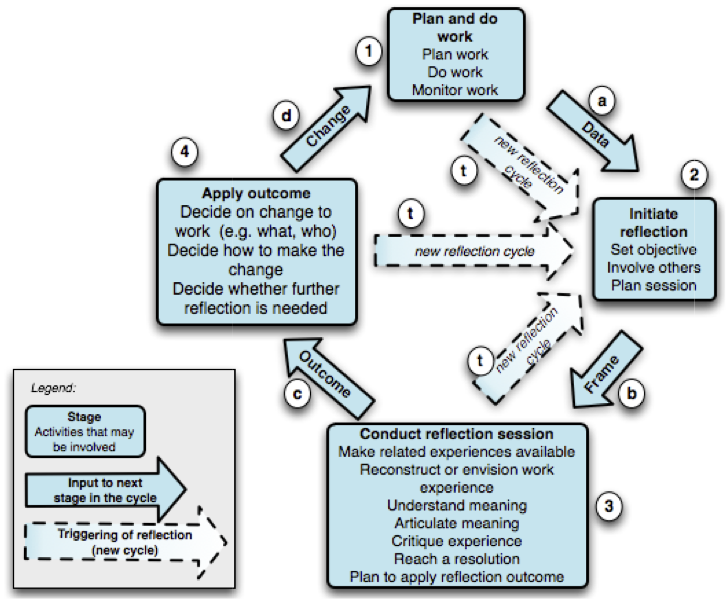
\includegraphics[width=1
	\textwidth]{CSRL} \caption{CSRL reflection cycle. Figure adapted from \protect\autocite{Krogstie:2013kf}} \label{fig:csrl-model-contrib} 
\end{figure}

During this PhD work two of the four stages of the model, \emph{plan and do work} and \emph{conduct reflection session}, have been instantiated and specific activities from each stage have been supported technology tools (Table \ref{tab:model-instantiation}). 

\begin{table}[tbh] 
	\centering 
	\caption{Instantiation of the CSRL model} 
	\label{tab:model-instantiation} 
	\smallskip
	\begin{tabular}{@{}P{0.15\linewidth}P{0.35\linewidth}P{0.20\linewidth}P{0.20\linewidth}@{}}
	\toprule
	Stage & Activity & Technologie & Prototype \\
	\midrule
	Plan and do work & Do work & Digital board game & \emph{Don't Panic} \\
	                 & Monitor work & Wearable computers & \emph{WATCHiT}  \\
	\hline
	Conduct reflection  & Make related experiences available & Mobile augmented  & \emph{CroMAR} \\
	session & Reconstruct or envision work experience & reality & \\
	& Understand meaning &  \\
	& Articulate meaning &  \\
	& Critique experience &  \\
	\bottomrule 
	\end{tabular}
\end{table}

During the \emph{plan and do work} the \emph{monitor work} and \emph{do work} activities have been supported. The \emph{monitor work} activity has been implemented by \emph{WATCHiT} (P3) which empowers workers for capturing a wide spectrum of qualitative and quantitative data. I found out that \textbf{wearable sensor technology and embodied user interfaces} provide the best design choice for data collection. The \emph{do work} activity has been supported by \emph{Don't Panic} (P4, P5), by generating realistic work experience that push workers towards taking actions common of real work and under stress conditions in a game environment. Although the \emph{do work} phase in the model describes real work activities, for the specific case of crisis management we claim it can also be applied to simulated work. Indeed, the innovative \textbf{digital board game technology} presented in P5 was effective in recreating stress conditions similar to real work and collaboration affordances typical tho the ones observed during field studies.

The \emph{Conduct reflection session} \emph{CroMAR} (P1) supports a wide range of activities. First it makes \emph{related experiences available} by aggregating data from multiple sources, including work experience of colleagues (captured by \emph{WATCHiT}), social networks and open data. Then \emph{CroMAR} allows for visualising data while being situated in a physical context that helps to \emph{reconstruct or envision work experience}. By allowing layering and filtering of data according to source, time and space it facilitates to \emph{understand and articulate meanings}. Finally an embedded text editor allows for the collection and sharing of lesson learnt and to elaborate a plan to apply reflection outcomes. Thanks to the experience with \emph{CroMAR} we also found out that \textbf{mobile augmented reality technology} is efficient in supporting debriefing and reflection after crisis work.

Contribution 1 can be a resource for researchers in the field of computer supported reflective learning that strive in finding solutions to map theory tools to technologies that people can use at work. Although the applications developed are tailored to the crisis training domain, they could be redesigned for other domains. The need for pervasive data collection and disruption-free interfaces is shared by many work practices; the digital board game approach developed in P5 has been proven to be a useful tool also in generating realistic work experience for the dementia care domain, as investigated during research work abroad (see Appendix \ref{abroad}). Finally a new application domain for mobile augmented reality technology: to support debriefing. \emph{CroMAR}, the tool developed in P1, could be adapted to support debriefing of work practices that share similarities with the crisis domain. The presented technology tools constitute an empirical evaluation of theory which outcomes (P2,P6) can inform future development of the CSRL model. Finally a new approach to the design of technology to turn unstructured context data into learning contents was presented in P6 and evaluated across two cases studies. The approach aims at extending the body of knowledge in computer-supported reflective learning.

\section{C2: Knowledge about designing experience-capturing tools for crisis workers}\label{c2-knowledge-about-designing-experience-capturing-tools-for-crisis-workers}

Contribution 2 of this thesis is a set of challenges for the design of experience-capturing tools during real or simulated crises.

Seven design challenges derived from multiple user studies with crisis workers, have been reported in P3. The challenges are summarised in Table \ref{tab:design-challenges}. Despite there are guidelines for designing sensor and capturing tools for a variety of domains; in this work I focused on capturing information that is is relevant for reflective learning in crisis training. The challenges shed light on \emph{what} information is relevant and \emph{how} to capture relevant information. This contribution also highlights a design trade-off common for many sensing-based applications: the degree of data that can be captured with sensors, automatically and without user intervention, versus information that can be submitted in-action by workers themselves; which, in the case of crisis training, requires novel interaction approaches (Contribution 3). 

The challenges have informed the design of \emph{WATCHiT}, a modular data capturing tool (P3) that has been successfully evaluated in a scenario to support debriefing after procedural training (P2). \emph{WATCHiT} can be configured to address new scenarios, data captured can be also used to support coordination of work or monitoring activities in real time.

Contribution 2 can be a resource for computer scientists aiming at designing technologies for pervasive quantitative and qualitative data collection. The presented challenges constitute a foundation for a design space for data capturing tools. They are an expression of the trade-off between technology-centred quantitative data acquisition and user-centred qualitative information collection.

\begin{table}
	[p] \centering \caption{Design challenges for data collection tools in crisis work} \label{tab:design-challenges} 
	\begin{tabular}
		{@{}p{0.05\linewidth}p{0.25\linewidth}p{0.60\linewidth}@{}} \toprule & Challenge & Description \\
		\midrule DC1 & Mobility of work and sensing & It is important to complement data from sensors embedded in the environment with mobile ones. The degree of mobility and thus granularity of data is important. Fine granular data is achieved with sensors worn by first responders. \\
		DC2 & Different crises, different relevant data & Being each crisis almost unique, it is difficult to define which data might be relevant to capture based on generic typologies of crises. \\
		DC3 & Different types of data & Different types of information are relevant to be captured. Including information for assessment of the worker’s safety, for mapping the territory and the work and Information related to the rescued people (e.g. type of injures). \\
		DC4 & Sensor data and user-submitted data & Workers might however provide critical qualitative data that cannot be measured with sensors to complement quantitative ones. \\
		DC5 & Different use, different sharing & While some types of data (e.g. location of agents) can be shared with colleagues to support real-time real time coordination, it's up each agent whether to share or not sensitive data (e.g. stress levels) with peers. \\
		DC6 & Intuitive, hands-free interaction & Workers must focus on the rescue operation and not on data capturing and logging tasks. User interfaces must be very intuitive and distraction-free. \\
		DC7 & Automate and discrete capturing & Capturing data with automatic means doesn't require user intervention but it produce datasets often affected by noise. Discrete capturing requires the user to activate sensors but produces more relevant and contextualised data. \\
		\bottomrule 
	\end{tabular}
\end{table}


\section{C3: Novel sensing-based interaction techniques to support recreation and generation of work experiences in crisis training}\label{c3-novel-sensing-based-interaction-techniques-to-support-recreation-and-generation-of-work-experiences-in-crisis-training}

Contribution 3 of the thesis brings novel interaction techniques to the field of sensing-based interfaces.

The interaction techniques developed assist different tasks.

During \emph{capturing work experience} the focus is on empowering users for collecting work experience without disrupting the work (due to interaction with the capturing tool). Building on prior works on mnemonic shortcuts \autocite{Guerreiro:2008wt} and body-centric interaction \autocite{Chen:2012wk} in P3 a novel disruption-free user interface is presented. It allows to use predefined body areas and objects as mnemonic shortcuts to activate sensors and to tag quantitative data with user-predefined information.

To enhance \emph{re-creating work experience} \emph{CroMAR}, the system presented P1, leverages mobile augmented reality (MAR) to enable visualisation and manipulation of reflection-useful information while being co-located in a physical context. In the implemented system the use of MAR technique has been proven successful in triggering reflection (P2). Moreover usability issues typical of MAR applications (e.g.~information overloading or occlusion visualising huge datasets) have been tackled by providing mechanism for filtering the information visualised according with time and source.

Finally during \emph{generating working experience}, tangible user interface frameworks have driven the design of the digital board game presented in P4 and P5. Board game mechanics have been functional to generate realistic work experience in terms of collaboration affordances and decision making. In this setting the use of tangible and sensing-based interaction added realism to the experience and increased players engagement and fun. The game design presented in P4 has been generalised in a approach and design process,presented in P5, that will drive the creation of future digital board games.

Contribution 3 can be a resource for interaction designers interested in creating interfaces for disruption-free data collection of experiences, situated data visualisation and simulated interactive experiences. The interaction techniques developed can be translated to new application domains.

\section{C4: Knowledge about implementing prototypes to be deployed into the wild}\label{c4-knowledge-about-implementing-prototypes-to-be-deployed-into-the-wild}

Contribution 4 brings new knowledge derived from the experience of the author in constructing prototypes of hardware and software systems. Prototypes were developed from the early phases of the research work to be used as demonstrator of tools for data collection (C2) and novel interaction techniques (C3). Also, ecologies of prototypes were functional for the evaluation of the CSRL model (C1), when more than one prototype was orchestrated in order to support part of the CSRL cycle.

Eight prototypes have been developed as part of this thesis. Each of them involved a mix of software, hardware and casing design. From a software point of view, the challenges consisted in making heterogeneous systems to discover each other and exchange data over a common protocol. This challenge has been addressed by the \emph{UbiDisco} middleware developed in P7. Most of the prototype featuring embedded hardware, I iteratively developed relatively complex electronics; for example to sense data from the environment or to provide haptic and visual feedbacks. I employed a wide range of technologies and toolkits which were not designed to be integrated, highlighting potentiality and limitations of state of the art technology for embedded systems. For example, the system of P5 involved the use of three different hardware toolkits and programming languages, and a bit of hacking. This attitude hacking and tinkering existing toolkits has been required because a product to fully fulfil the implementation of requirements of our system was not available on the market. Yet this is a resource for hardware engineers willing bring advances in the state of the art of toolkit for building electronics.

Prototypes used by crisis workers, in-action, have to be built for higher resilience compared to digital artefacts developed for lab testing. The simulated rescue work activities in which we staged our systems' evaluations are designed to recreate conditions as close as possible to real emergencies; including exposure to physical and thermal shocks. This setting has required the prototyping process to move one step closer to product engineering. The final stage of prototypes feature 3D-printed and laser-cut enclosures to shelter the electronics from the environment. Moreover for iteration after iteration the size of the prototypes has shrunk. For example the system in P3 have reached in four iterations a size compatible for being comfortably worn underneath work uniforms.

Contribution 4 is a resource for hardware and software engineers. Also it serves at case study for researcher to investigate the design of hardware and software toolkits to assist prototyping of electronic inventions. 
